% \documentclass[]{diss}
% \begin{document}

\chapter{Introduction}
% German locative phrases
Spatial language is a vast topic. This book focusses on locative phrases, 
which are phrases that single out objects in the physical environment with the 
\emph{communicative intention} 
to draw attention to these objects. The following shows an example
of a locative phrase from German.
\ea
\label{e:der-block-rechts-der-kiste-von-dir-aus}
\gll der Block rechts der Kiste von dir aus \\
the.{\NOM} block.{\NOM} right.{\PREP} the.{\GEN} box.{\GEN} from.{\PREP} your.{\DAT} perspective \\
\glt `The block to the right of the box from your perspective'\\
\z

% highly developed tool
Phrases like this can be seen as highly complex tools that help dialog 
partners to establish spatial reference. The utterance conveys to the hearer 
a number of instructions such as (1) apply the spatial relation {\footnotesize\tt right},
(2) use a particular landmark and (3) take the perspective of the interlocutor.
These instructions, when applied properly, allow an interlocutor 
to identify the object in question. The syntactic structure, i.e. the words and the 
grammatical relations of the utterance, encode
which concepts and categories should be used and how the instructions work together. 
For instance, the fact that the hearer's perspective on the scene should be taken
is conveyed by the phrase \textit{von ... aus} (`from ... your' perspective).

% cross-linguistic variation
Languages vary widely in how they solve the problem of spatial reference --
including both how they conceptualize space and how they
talk about it \citep{levinson2006grammars,levinson2003space}\index{Levinson, S. C.}\index{Wilkins, D.}. 
Spatial position of objects can be expressed using 
a variety of syntactic means including case, 
adpositions, particles, and verbs. But, maybe more importantly, 
there is a breathtaking variety in how people conceptualize space,
which spatial relations they know, what counts as a landmark, how
perspective is used, etc. Just to give a few simple examples, Spanish has
three basic proximal distinctions, while German has two.
In Barcelona people make active use of the topology of
the surrounding landscape, referring regularly to the
seaside and mountainside when giving navigation instructions. 
In other languages \emph{uphill} and \emph{downhill} 
are used to refer to proximal objects \citep{levinson2003space}\index{Levinson, S. C.}.

%% highly specialized tool 
These examples show that spatial language is a highly developed tool for 
establishing reference in a spatial environment. How did spatial language 
become this way? There is an emerging view now that the most plausible answer 
to this question is that spatial language is a \textsc{complex adaptive system}\index{complex adaptive system}
(see \citealp{steels2000language}\index{Steels, L.} for the general idea of language as a complex adaptive system), 
that is constructed and changed by its users for the same purpose it is used for today, 
namely to describe spatial scenes,
establish reference to objects in the environment, give instructions for navigation, etc.
This process is, of course, not the same process of construction that a group
of engineers use when they are building a bridge. In such classic engineering
problems, a team of people with a more or less complete view of the problem
designs a top-down solution. By contrast, nobody has a global view on the state 
of a language. Rather, language lives in the individuals of 
the language community. Every individual has 
its own views on the state of the language, i.e. what words and 
grammatical relations are available.

% complexity -> look to biology
When we combine the evidence from the complexity of particular spatial languages,
such as German locative phrases, and the variation that can be seen across 
languages, it seems reasonable to consider results from a science 
that routinely deals with complexity and variation -- biology. Biological species are highly 
complex solutions to particular environmental and social challenges. The solutions
found by each species exhibit a high degree of variation. This simple observation has
forced biology to come up with precise models and predictions to explain the 
origins of species. It comes as no surprise, then, that theories of language, particularly 
language evolution and language change, have adopted concepts 
from biology related to variation, complexity and the emergence of order 
in biological systems.  

% selectionist theory of language evolution
This book defends the \textsc{selectionist theory of language evolution},
which exploits biological concepts to explain how language is shaped 
by the communicative needs and environmental conditions that a 
community or population faces. 
The theory hypothesizes that agents create variation within their language 
and select working solutions based on how successful they are 
in communication (\textsc{communicative success}), 
how complex they are in processing (\textsc{cognitive effort}) and 
other factors. 

% whole systems approach
Studying language change from the perspective of communicative
intentions requires a great deal of insight into how humans or artificial 
systems can realize their specific communicative intentions 
in social interactions in the physical world. Such holistic explanations 
necessitate a \textsc{whole systems approach}\index{whole systems approach}
\citep{steels2001language}\index{Steels, L.},
in which great care is taken to ensure that perception, conceptualization 
and linguistic processing systems are integrated to an extent that 
interaction between agents is possible. Only when all of this machinery is 
in place can one attempt to examine questions of language change.

% operational models
In particular, a whole systems approach requires an operational theory of 
language. How are utterances processed? How is space conceptualized?
How is linguistic knowledge represented? How does language
interact with the perception of the physical reality? A whole systems approach 
requires concrete answers to each of these important questions. The resulting 
burden placed on operational models is of course far greater than for high-level 
explanations or logical reasoning about these processes. But concrete, 
mechanistic accounts allow much greater insights into the phenomena studied.
In the best case, a successful model of language evolution in a whole systems 
approach validates many aspects of the theory of language and language 
change at the same time.

% contributions
This book contributes to the understanding of spatial language in two ways. 
First, it provides a detailed operational reconstruction of German locative phrases
using a whole systems approach. Second, it explores the evolution of spatial
language within the same computational framework. The two parts  
together argue for (1) the validity of the approach to language, and (2) the validity
and explanatory power of the selectionist theory of language evolution.


%%%%%%%%%%%%%%%%%%%%%%%%%%%%%%%%%%%%
\section{Locative spatial language}
\label{s:intro-spatial-language}
If one wants to make an interesting claim about how language evolves, one needs a
solid idea what language actually is, how linguistic knowledge is represented, and
how to organize linguistic processing. These questions are best answered
by reconstructing a complex natural language phenomenon such as German locative 
phrases. Such phrases are used for establishing reference to 
static objects and identifying them by denoting their spatial position \citep{miller1976language}\index{Johnson-Laird, P. N.}\index{Miller, G. A.}.
They can be distinguished from other parts of spatial language
that are dealing with motion or navigation \citep{eschenbach2004functional}\index{Eschenbach, C.}. 

German locative phrases can be analyzed in terms of components 
or systems which together form a locative phrase. Example 
\ref{e:der-block-rechts-der-kiste-von-dir-aus} consists of three parts: 
a \textsc{spatial relation}, which is combined with a \textsc{landmark} and 
a \textsc{perspective}.

\begin{description}
\item[Spatial Relations] The defining quality of locative spatial phrases
are that they contain locative spatial relations such as 
\textit{rechts} (`right'), \textit{vorne} (`front'), \textit{nah} (`near'), 
\textit{n\"ordlich} (`north on' and so forth).
These relations are called locative because they encode
static spatial relationships and do not refer to change of position in time. 
In the Example phrase, \textit{rechts} (`right') is the locative spatial relation.
In this book we study three classes of spatial relations. 
\emph{Proximal} relations are based on distance estimations. 
Examples of proximal relations in German are \textit{nah} (`near') and \textit{fern} (`far').
The second class is called \emph{projective}
relations and includes direction-based spatial relations such as \textit{links} (`left') and \textit{vor} (`front').
The last class considered are absolute relations such as \textit{n\"ordlich}
(`north') and \textit{\"ostlich} (`east'). These are also direction-based, but the direction
is related to a geocentric reference system such as the magnetic poles of the
earth.
\item[Landmarks] A spatial relation is at least a binary and always
relates to something. This something is typically called \emph{landmark}.
In \REF{e:der-block-rechts-der-kiste-von-dir-aus}, the landmark 
is expressed in the determined noun phrase 
\textit{der Kiste} (`the box') immediately following the spatial relation.
\item[Perspective] For certain spatial relations perspective is important.
Example \ref{e:der-block-rechts-der-kiste-von-dir-aus} features a 
perspective that is marked via the phrase \textit{von ... aus} (`from ... viewpoint').
The marker expresses that the viewpoint on the scene is the hearer. 
\end{description}

%%%%%%%%%%%%%%%%%%%%%%%%%%%%%%%%%%%%
\section{A theory of language evolution}
\label{s:intro-evolutionary-linguistics}
Theories of language evolution have to explain the evolution of language
by defining the role and contribution of four different factors on language:
biology, cognition, social cognition, and culture 
\citep{steels2009cognition,steels2011self-organization}. 

\begin{description}
\item[Biology] To study language evolution from the biological
perspective is to ask questions about the relationship of biology,
in particular, genetics and ecology with linguistic behavior.
The question can be roughly split into two parts.
First, what is the biological influence on the general capacity for language
in the human population? Second, one can ask for the influence of biology on 
the particular language spoken by individuals. The first is a general question for 
the processing capabilities that need to be present for language.
This includes that humans require sufficient memory and powerful neural 
circuitry for processing language, but also production organs for speech 
and auditory capacities. The second question is how much the biological basis 
determines the particular language individuals speak. 
In other words, how much the lexicon and/or the grammar
of a language are influenced by genetic conditions. 

\item[Cognition] Biology has provided us with neural 
circuitry that enables distinct cognitive capabilities.
The cognitive perspective on language asks: what are the basic cognitive 
processing mechanisms underlying production and parsing of language, 
interpretation, conceptualization, but also categorization, perception
etc.? Language depends on a number of capabilities that may or may 
not be prior to language, such as temporal clustering 
of events, spatial navigation, perception-action systems 
\citep{rizzolatti1998language,arbib2002mirror,steels2012mirror,steels2008mirror}\index{Arbib, M. A.}\index{Rizzolatti, G.},
memory and so on and so forth. For instance, some have linked the evolution 
of language to an increase in capacity for storing cognitive categories and 
their interrelations \citep{schoenemann1999syntax}\index{Schoenemann, P.}. Another 
strand of cognitive influences on language evolution are general 
cognitive operators such as analogy and
learning operators, for instance sequential learning 
\citep{christiansen2001sequential}\index{Dale, R.}\index{Christiansen, M. H.}\index{Ellefson, M. R.}\index{Conway, C. M.}.

\item[Social Cognition] Inevitably, language is a social phenomenon that
occurs when humans interact. Social cognition researchers, for instance, 
are interested in the social mechanisms that are needed for children to acquire 
language, but also in the social mechanisms that are prerequisite for the emergence of language.
Proposals include things such as \emph{theory of mind} \citep{dunbar1998theory}\index{Dunbar, R.} which
is the capacity to understand another individual's state of mind, 
\emph{joint attention}\index{joint attention} \citep{carpenter1998social}\index{Tomasello, M.}\index{Nagell, K.}\index{Carpenter, M.}\index{Butterworth, G.}\index{Moore, C.}
which is the ability to track interlocutor gaze and mutual 
attentiveness to the same object, \emph{social learning skills}\index{social learning skills} such as imitation learning 
\citep{tomasello1992social}\index{Tomasello, M.} and the ability and the urge to \emph{share intentions}\index{shared intentions} 
\citep{tomasello2005understanding}\index{Call, J.}\index{Carpenter, M.}\index{Moll, H.}\index{Tomasello, M.}\index{Behne, T.}. Many of these mechanisms are deeply rooted in biology.
For instance, \cite{dunbar2003social}\index{Dunbar, R.} and \cite{worden1998evolution}\index{Worden, R.} argue that
theory of mind is a necessary preadaptation for language and that it has 
evolved via natural selection\index{selection}.

\item[Culture] Language is a cultural phenomenon that is undergoing 
steady change on the cultural level. New words, speech sounds, morphemes,
semantic and syntactic structures arise all the time in language \citep{steels2011self-organization}.
This manifests in the incredible amount of cross-cultural variation
on all levels of linguistic processing \citep{evans2009universals}\index{Levinson, S. C.}\index{Evans, N.}, for example, phonemes 
\citep{maddieson1984patterns,oudeyer2005self}\index{Oudeyer, P. Y.}\index{Maddieson, I.}, spatial semantics \citep{levinson2003space}\index{Levinson, S. C.},
and syntax \citep{levinson2006grammars}\index{Levinson, S. C.}\index{Wilkins, D.}. 
This evidence points to strong cultural negotiation processes in which continuous invention 
is channeled to produce complex useful communication systems.
Many of such processes orchestrating change and diversification have been identified.
Grammaticalization, for instance, tries to explain the shift from
lexical items to grammatical items \citep{hopper2003grammaticalization}\index{Hopper, P. J.}\index{Traugott, E. C.}.
Others have pointed to generational change as the trigger for 
development in language \citep{smith2003iterated}\index{Brighton, H.}\index{Smith, K.}\index{Kirby, S.}.
The question from the perspective of cultural evolution is what are the mechanisms 
that bring about change in language and what are the principles with
which agents conventionalize language up to the point that interlocutors 
have a chance of understanding each other.
\end{description}


I emphasize the cultural point of view in this book. That is, my primary concern is
with change in language on the cultural level independent of changes in the human 
biology. Language change occurs on a smaller time scale than, for instance, the 
adaptation of a new biological organ, let alone a new species. There is absolutely no 
doubt that languages evolve fast. One just has to look through a text by 
Shakespeare or Goethe to see that a few hundred years can have impact
on vocabulary and grammatical structure. It took Vulgar Latin a mere 1500 years to 
evolve into about a dozen different languages such as French, Italian, 
Portuguese or Catalan (e.g., see \citealp{pope1952latin}\index{Pope, M. K.} for French). 
If we observe languages today, we can easily see 
that new words are invented all the time.
In academic and technological contexts, for instance, new concepts arise all the time.
Roughly 30 years ago vocabulary such as \textit{email} or \textit{website} did not even exist.
What drives change in language, in what circumstances does it take place and 
what are necessary requirements for language change to occur? These are questions 
that cultural evolution theories of language have to address.

\subsection{Language Systems and Language Strategies}
Cultural theories of language evolution have to take a close look at individual 
trajectories of language change \citep{steels2011self-organization}. For instance, 
how did the Russian aspectual system emerge or why does English have a
system of determiners and Russian not? How do spatial language systems 
develop over time? In other words, cultural theories of language
evolution must provide models for the emergence and evolution of concrete
\emph{language systems} \citep{steels2011self-organization}. \index{language system}\index{language strategy}
Language systems package a particular 
\emph{semantic system} (e.g. a set of spatial categories) and a 
particular way of expressing these distinctions (e.g. a corresponding set of 
lexical items). The absolute German system, for instance, consists of 
four absolute spatial categories and the corresponding strings, e.g. 
\textit{n\"ordlich} (`north'), \textit{s\"udlich} (`south'). These spatial
categories are the basic building blocks of absolute spatial conceptualization 
in German. They can be compositionally combined with landmarks to
build complex spatial phrases. Interestingly, the 
German locative systems effectively consist of different conceptualization
strategies that have distinct but converging evolutionary trajectories. For instance,
the absolute system is connected to the invention of the compass,
whereas projective systems often at least in part can be traced back to 
body parts \citep{traugott1991grammaticalization}\index{Heine, B.}\index{Traugott, E. C.}.
Nevertheless, many locative spatial relations are used in the same syntactic 
context.

Spatial language systems such as the proximal or projective system 
are characterized by a degree of cohesion and systematicity 
that points to an underlying principle that organizes acquisition, emergence 
and coordination. We call the mechanisms organizing a particular language
system the \textsc{language strategy} \citep{steels2011self-organization}.
Language strategies have a \emph{linguistic} and a \emph{conceptual} 
part. For example, on the conceptual 
side absolute spatial categories share that they
are part of the same conceptualization strategy which uses absolute directions
to the magnetic poles of the earth. Syntactically all spatial relations share
that they are expressed in a similar way namely lexically and that they can
be expressed as adjective, adverb and preposition. 


\subsection{Selectionist Theory of Language Evolution}
In this book I follow the \emph{selectionist theory of language evolution} 
\citep{steels2011self-organization}, which applies the dominant theoretical construct 
in biology \emph{natural selection} and uses it to explain language change\index{selection}
on the level of \emph{language systems} and \emph{language strategies}.
Additionally, the concepts of \emph{self-organization}\index{self-organization},
\emph{recruitment}\index{recruitment} and \emph{co-evolution}\index{co-evolution} of syntax and semantics are
used as theoretical pillars.

\begin{figure}
\begin{center}
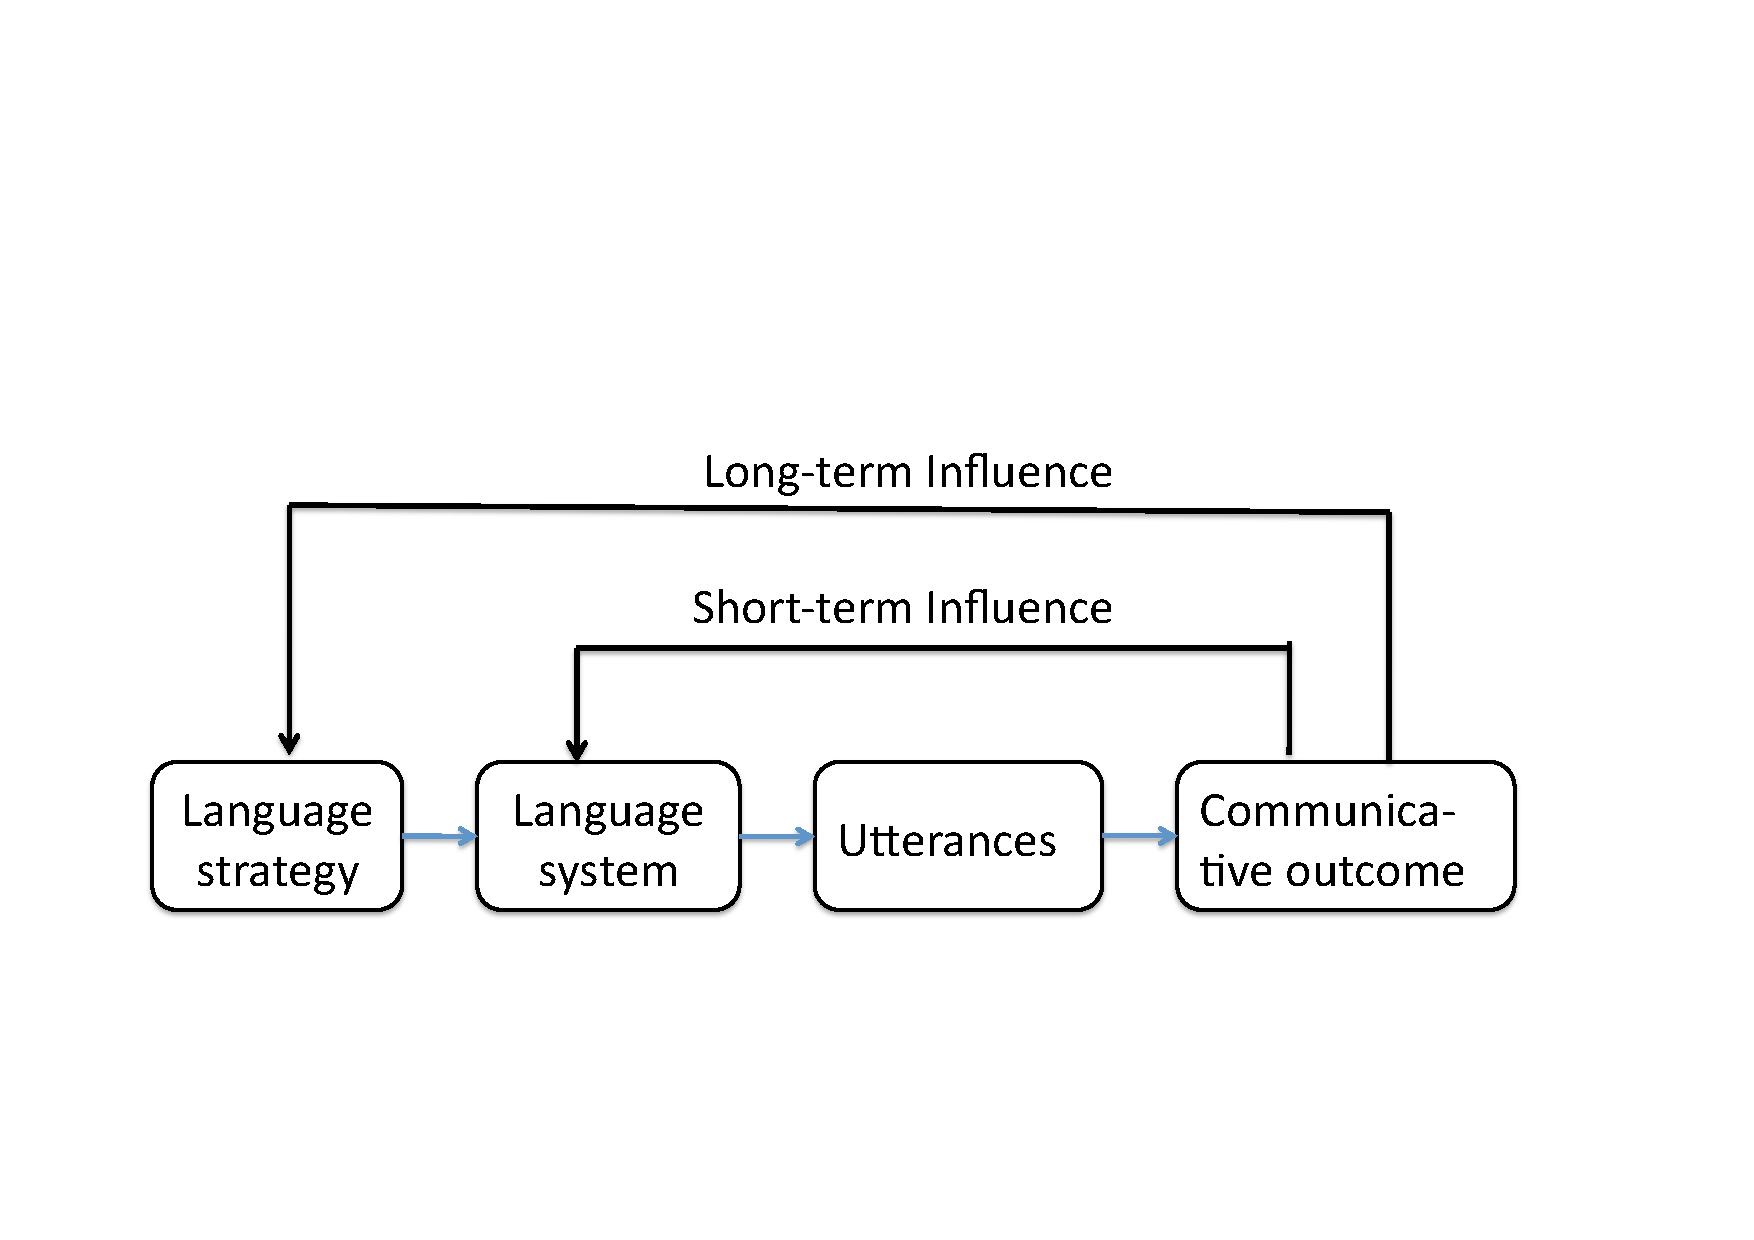
\includegraphics[width=0.7\columnwidth]{figs/select-strat}
\end{center}
\caption[Selective pressures on language systems and strategies]{The fitness of utterances for communication affects both the language
system and the language strategy. The effect of the success of a single utterance 
on the language strategy is smaller which leads to slower change on the level 
of the strategy. (Figure adapted from \citealp{steels2011self-organization})}
\label{f:strategy-system-selection}
\end{figure}



\begin{description}
\item[Selection]\index{selection}
Selectionism rests on two principles: \emph{generation} of
possible variants and \emph{selection} of variation based on fitness. 
The most important factor in determining the fitness of a 
particular language strategy, but also
of a particular language system, is \emph{communicative success}.
A communicative interaction between two interlocutors is successful if the
communicative intention of the speaker is reached. For instance, if the speaker
wanted to draw attention to some object, the communication is successful if the
hearer pays attention to that object. Communicative success drives selection\index{selection}
on the levels of the language system, but also on the level of language
strategies (see Figure \ref{f:strategy-system-selection}). 

Variation occurs in the systems for two reasons. 
First, agents are actively trying to solve 
problems in communication \citep{steels2000language}\index{Steels, L.}. 
Agents introduce new categories, 
new words and grammar when they detect problems that they 
cannot solve using the current
language they know. Second, language is an inferential 
communication system \citep{sperber1986relevance}\index{Wilson, D.}\index{Sperber, D.} which means 
that the information provided in an utterance is often 
incomplete and ambiguous. Interpreting phrases is an active 
process in which the hearer
is fusing information from the context, from the dialogue 
and his knowledge about the language 
to arrive at the best possible interpretation. In this process 
of course hearers might interpret
the utterance differently then intended. This is the 
second source of variation.

\item[Self-organization]
\cite{steels2011self-organization}  assumes that selection\index{selection} is not enough to explain 
language change and proposes another driving force in the evolution of language: 
self-organization\index{self-organization} -- a concept used to account for complex 
phenomena in physical and biological systems. In short, self-organization is a way to explain 
how global structure arises out of local interaction of subunits \citep{camazine2003self}\index{Camazine, S.}\index{Franks, N. R.}\index{Bonabeau, E.}\index{Sneyd, J.}\index{Deneubourg, J. L.}\index{Theraula, G.}. 
An example from biology for self-organization is swarm behavior in a school of fish. 
Each individual fish locally controls its behavior based on the estimation of the 
position and direction of its immediate neighbors. On the global level this leads to 
consistent swarm behavior. Self-organization is typically seen as a complementary 
mechanism to selection\index{selection}, although there is some discussion 
on how to reconcile the two mechanisms. 
\cite{kauffman1993origins}\index{Kauffman, S. A.}, for instance, proposes the following idea. 
Local components and the interaction rules are determined by selection\index{selection}, whereas the global emergent behavior is explained using self-organization. 
Applied to the swarm behavior this means that the anatomy of fish as 
well as the perceptual feedback loop are a product of natural selection. 
The global emergent swarm behavior is the product of self-organization. \index{selection}

Similar to swarm behavior, agents in a population evolving a language have
to achieve global coherence in the language they use. Each agent has its own 
private representations of the language that they speak and they can 
adjust their own representations based on local interactions with peers. 
How, from local interactions, agents can agree
on a globally shared communication system is the problem of alignment\index{alignment}.
Psychologists have found that interlocutors align on all levels of linguistic processing
even over the course of a few interactions, i.e., dialogue
\citep{garrod1994conversation,pickering2004toward}\index{Garrod, S.}\index{Doherty, G.}\index{Pickering, M. J.}.
Similar mechanisms applied over a long time span are required for driving populations 
to self-organize a sufficiently shared communication system 
\citep{steels2002bootstrapping}\index{Steels, L.}\index{Kaplan, F.}. 

\item[Recruitment]\index{recruitment}
The last problem for an account of how languages change in the 
\emph{selectionist theory of language evolution} is the problem of language strategy
generation. The hypothesis is that language strategies are recruited by assembling
basic cognitive operations\index{cognitive operation} \citep{steels2007recruitment}\index{Steels, L.}. For instance, an 
absolute spatial conceptualization strategy\index{conceptualization strategy}
involving distinctions such as ``north'' and ``south''  consists of basic categorization
mechanisms and the ability to track ones own direction. The two abilities are assembled
into the strategy which encompasses the different absolute spatial distinctions.
The process is called \emph{recruitment}\index{recruitment} because the cognitive mechanisms which
are assembled could, in principle, have evolved or could be learned independently 
from language. 

\item[Co-evolution] \index{co-evolution}
One of the tenants of the theory of linguistic selection is that syntax and semantics co-evolve. 
The idea is that recruitment\index{recruitment} of conceptualization strategies and the invention of new
semantic distinctions and spatial relations trigger evolution of the syntax of a language
\citep{steels1997distinctions,steels1998synthesizing}\index{Steels, L.}.  
For instance, presumably when the absolute system in German emerged based
on a new way of construing reality, this at the same time triggered 
the invention of new words. 
\end{description}

\subsection{Evolutionary explanations}
In every science one has to define what counts as an explanation. 
This book is guided by what counts as an evolutionary explanation
in biology, ethology and psychology \citep{tinbergen1963aims,dunbar1998theory}\index{Tinbergen, N.}\index{Dunbar, R.}. 
In order to explain a complex trait from the evolutionary perspective 
one has to provide explanations on four different levels: \emph{function}, 
\emph{mechanism}, \emph{ontogeny} and \emph{phylogeny}.

\index{function}\index{ontogeny}\index{phyologeny}\index{mechanism}
\begin{description} 
\item[Function] An explanation for a particular behavior has to show what
the behavior is good for, i.e. what is its purpose. For Darwinian biology, 
the function of a behavior has to be explained in terms of its impact 
on survival or, more precisely, on the production of offspring. For evolutionary
linguistics this turns into the question of how a particular language system or a particular strategy
helps an agent to be more successful in communication. For example,
one can explain particular spatial language systems with respect to their ability
to help agents solve communicative problems in spatial navigation and 
spatial reference.

\item[Mechanism] Besides function, one has to identify the mechanisms that give rise 
to the behavior. 
This is actually called \emph{causation} by \cite{tinbergen1963aims}\index{Tinbergen, N.} 
and it refers to the cause and effect relations that generate a particular behavior. 
For instance, one can explain how aggressive behavior is generated by looking
at changes in hormone levels in an organism, e.g., testosteron causes aggressive behavior.
For spatial language this entails a detailed operational model of the 
production and parsing of spatial language.

\item[Ontogeny] The next question is how a particular behavior is acquired. To
answer this question one has to identify the developmental steps that
the behavior undergoes, but also what is the ontogenetic basis 
of the behavior. What is learned and what is instinct? For spatial language this 
requires insights into how spatial language is learned.

\item[Phylogeny] A fourth part of every evolutionary explanation has to
identify the evolutionary history of a behavior. What are
the sequential stages of evolution of a behavior? What are the prerequisites
of a behavior? How do evolutionary older behaviors influence 
the behavior under question? These questions have to be answered
with respect to the function of the behavior. In other words, one needs
explanations of how the behavior evolved to fulfill its current function. 
For language evolution scholars have to identify how a particular strategy 
evolved over time. Was it adapted from an older strategy? 
How did syntax and semantics of the language system under consideration co-evolve over time?
\end{description}

\section{Main hypothesis}
\label{s:intro-main-hypothesis}
This book provides experimental evidence for the theory of linguistic
evolution. The hypothesis is that \emph{spatial language syntax and 
spatial semantics co-evolve through a cultural process based on selection\index{selection}, 
self-organization and recruitment}\index{self-organization}\index{recruitment}. This book explores the hypothesis for 
the different components of spatial language: spatial relations, landmarks 
and perspective. Computational experiments
show the emergence of spatial relations, the negotiation of the use of landmarks
and perspective. I also explore different strategies for expressing
spatial conceptualizations: lexical and grammatical strategies.

\section{Contributions}
\label{s:intro-objectives}
This book provides detailed accounts of 
the function, mechanisms, ontogeny and phylogeny of spatial language. 
\begin{enumerate}
\item The first contribution is an explanation of the mechanisms behind spatial language
for German locative phrases in a complete reconstruction including
perception, semantic and syntactic processing. Once the mechanisms are in place,
we test the function and impact of components of spatial language in experiments
by removing the component in question and examining the effect the removal has
on communication.
\item The second contribution is to explain steps in the co-evolution\index{co-evolution} of spatial 
syntax and spatial semantics through computational models.
\end{enumerate}

This book follows a whole systems approach which allows us to define external 
criteria for the progress in each of the objectives. The defining moment for the 
underlying conception of language is communication. A communication system 
is \emph{successful} if it allows robotic agents to achieve 
their communicative goals such as drawing the attention to an object in the environment. 

% steps in the evolution of spatial language
\subsection{Evolutionary Stages}
\label{s:stages}
One way of understanding evolutionary processes is to try to identify
evolutionary stages. Over the years, different steps in the evolution
of language have been identified involving varying degrees of 
specificity \citep{bickerton1999language,jackendoff1999possible,steels2005emergence}\index{Steels, L.}\index{Jackendoff, R.}\index{Bickerton, D.}. 
All of these proposals, while differing in detail and the exact number of stages,
agree that language evolution starts at some pre-grammatical stage and 
increases in complexity to the form of language, in particular, grammar 
that we see today. Obviously any evolutionary account of language has to show how 
the current state of complexity of language can be traced back to earlier simple stages. 


\begin{figure}
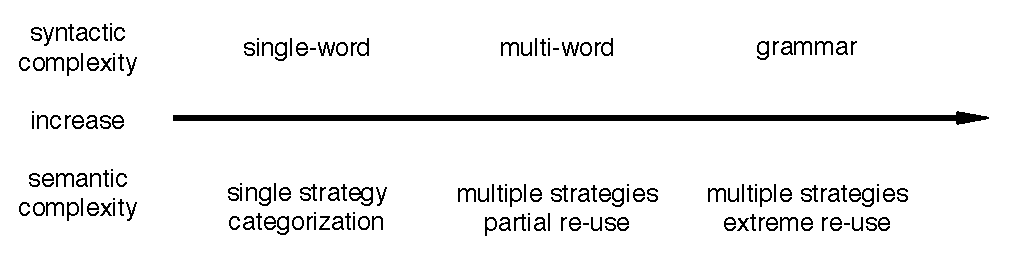
\includegraphics[width=1\columnwidth]{figs/co-evolution-complexity}
\caption[Co-evolution of syntactic and semantic complexity.]{Co-evolution\index{co-evolution} of syntactic and semantic complexity.}
\label{f:co-evolution-complexity}
\end{figure}

This book orients itself alongside \cite{steels2005emergence}\index{Steels, L.}, who proposes
a number of stages of complexity which are relevant for this book:
\emph{single-word utterances}, \emph{multi-word utterances}, and \emph{grammatical utterances}
(see Figure \ref{f:co-evolution-complexity}). 
 
\begin{description}
\item[Single-word utterances] In this stage agents utter single words that pertain to a particular concept
or category used for discriminating objects. Examples for spatial language include utterances that 
directly refer to spatial regions such as \textit{links} (`left') or \textit{n\"ordlich} (`north').
When agents can only express themselves using a single word, this single word necessarily encodes
the complete conceptualization strategy. For instance, which landmark or perspective is used for conceptualization is holistically coded in the single word. Since there is no additional information 
about which conceptualization strategy the term is referring to, agents have to implicitly agree on 
the precise spatial construal the term is referring to. This limits the re-use of spatial categories 
in different spatial conceptualization strategies because agents have no way of 
disambiguating the use of the same spatial relation in different strategies.
\item[Multi-word utterances] Single-word communication systems are not very flexible. 
There is no compositionality and particularly there is no re-use. In German, for instance,
projective relations can be used with different landmarks. In the multi-word utterance stage 
agents can express different constituents by using a number of lexical items. 
Besides expressing the spatial category used, agents can also 
mark landmarks. An example utterance is \textit{links Kiste} (`left box') which is used 
to signal that the region left of the box is meant.
\item[Grammatical utterances] When we look at natural language, we can see 
that the \emph{same} constituents can be part of different conceptualization strategies. 
Imagine an utterance like \textit{Kiste link} (`box left') without the grammatical information, in particular, 
without word order and lexical class information. In that case a hearer does not know whether 
\textit{link} is an adjective or an adverb. This syntactic underdetermination has consequences for 
the semantic interpretation. If the phrase is interpreted as an adjective noun phrase as in 
\textit{linke Kiste} (`left box'), the spatial category acts as a modifier on the set of boxes. If the 
spatial relation is interpreted as an adverb, then box might be a landmark and the whole phrase 
denotes a region next to the landmark as in \textit{links der Kiste} (`to the left of the box').
Grammar signals the difference in these two semantic interpretations and
disambiguates the conceptualization strategies. Consequently, agents equipped with grammatical
strategies can disambiguate even more strategies and consequently, they can be more expressive.
\end{description}

The goal of this book is to identify, implement and test the mechanisms that drive 
the evolution of language on \emph{each} of these stages. The mechanisms 
we are interested in are not descriptions of the phenomena but mechanistic explanations 
which identify the computational and cognitive components
that enable robotic agents to self-organize communication systems.
The procedure to find and validate mechanistic explanations is to
\begin{enumerate} 
\item hypothesize \emph{invention}, \emph{adoption} and \emph{alignment}\index{alignment} operators for the syntax and semantics
according to each stage of complexity,
\item equip agents with these operators,
\item test the evolutionary dynamics in populations of equipped agents,
\item measure the communicative success, adaptivity and expressivity.
\end{enumerate}
\index{invention}\index{adoption}
Invention, adoption and alignment\index{alignment} operators are the backbone of the evolutionary models 
of this book. For instantiating the theory of linguistic selection\index{selection} one has to identify 
agent-level mechanisms that orchestrate the global behavior of the population. The mechanisms 
can be classified into the following three classes.
\begin{description}
\item[Invention operators] Invention is the process of introducing variation 
into the system by inventing a new spatial relation or a word or even grammar
in order to solve a problem in communication. A speaker, for instance,
who is unable to discriminate an object might introduce a new spatial
category to be able to identify the object. Subsequently, he might invent
a new word to be able to express the new spatial category.
Invention operators introduce variation and novelty into the system.
\item[Adoption operators] Adoption is the process by which an
agent acquires a new word, a new spatial relation or a new piece of grammar.
Acquisition is carried out by hearers in interactions when they observe
new items that they are unable to process.
Adoption is another source of novelty and variation. An agent that
picks up a new word might have a different idea of what that word
means than the speaker actually intended. 
\item[Alignment operators] Invention is local to an interaction. When two
agents communicate and one of them invents a new word, this word
might be acquired by the interlocutor, but the knowledge about this 
word is still local. Alignment\index{alignment} operators orchestrate the self-organization\index{self-organization}
of the system and the global alignment of language.
\end{description}


\subsection{Co-evolution of syntactic and semantic complexity}
In each stage, syntactic complexity co-evolves\index{co-evolution}
with semantic complexity (see Figure \ref{f:co-evolution-complexity}). 
Syntactic complexity rises because the number of words
per utterance increases (from the single-word stage to the multi-word stage) 
and because syntactic categorizations such as word order, morphology, 
agreement become important (from multi-word to grammar).

The notion of semantic complexity is harder to define. Obviously
German spatial language is complex. But why does this seem obvious? 
What are the properties that make it a complex semantic system? For this book, 
complex semantics is defined with respect to spatial language as: the language supports a large 
number of conceptualizations of a spatial scene. There are two factors influencing 
the complexity of the space of possible conceptualizations of a spatial scene.

\begin{description}
\item[Number of relations] A first level of semantic complexity
is related to the number of spatial categories. For the part
of German locative phrases considered in this book, we already have 
12 spatial relations. But there are, of course, many more relations not considered
in this book such as  dynamic relations. 
For some scholars this is the only definition of semantic complexity (compare 
\citealp{schoenemann1999syntax}\index{Schoenemann, P.}).
\item[Number of conceptualization strategies]
A second notion of semantic complexity is the number of
conceptualization strategies a language supports. German, for instance, supports
many different categorization systems: projective, e.g. \textit{links} (`left') or \textit{rechts} (`right'), 
proximal, e.g. \textit{nah} (`near') and \textit{fern} (`far'), and absolute, e.g. \textit{n\"ordlich} (`north') 
and \textit{s\"udlich} (`south'). This is one aspect. The other aspect is that
these systems are part of different conceptualization strategies. 
Examples of this re-use were already given earlier with respect to adjectives and adverbs.
\end{description}

\section{Structure of the book}
\label{s:intro-structure}
This book is structured into three main parts besides this introduction 
and the conclusion. Part \ref{p:embodied-language-games} explains the interaction
model and the technical systems needed for studying spatial language.
Part \ref{p:german-locative-phrases} deals with objective number one and details the reconstruction
efforts for the German locative system. In Part \ref{p:spatial-language-evolution} I detail how spatial
language evolves based on the model of evolutionary stages.


\subsection{Part I: Spatial language games and technical background}
\index{spatial language game}
\subsubsection{Spatial language games}
Spatial language occurs mainly in interactions of individuals in spatial scenes.
To research spatial language in such a communication-based approach
to language a number of things need to be in place. We need a model of 
interactions in spatial scenes. This is the topic of Chapter \ref{s:spatial-language-games} which 
introduces \emph{spatial language games} which are routinized interactions
consisting of defined roles for interlocutors -- speaker and hearer. 
The chapter explains the basic interaction scheme and the 
linguistic and non-linguistic behaviors that define a spatial language
game. 

\subsubsection{Embodied cognitive semantics with IRL}
In order to achieve the objectives of this book, we need computational 
formalisms that support the reconstruction and evolution investigations. 
One of such formalisms in part developed for this book is the
\emph{Incremental Recruitment Language} (IRL). IRL is (a) a formalism
for representing semantics, (b) a set of planning algorithms for automatic
conceptualization and interpretation, and (c) a set of tools that make
semantics an open-ended adaptive system. Chapter \ref{s:irl} 
introduces the formalism and the technology behind it.

\subsubsection{Construction grammar with FCG}
Another important backbone of the investigations is Fluid Construction 
Grammar (FCG). FCG is a formalism for representing and processing linguistic 
knowledge. Chapter \ref{s:fcg} details how mappings from semantics to syntax 
are implemented using FCG and gives an example of processing a simple phrase.\index{Fluid Construction Grammar}

\subsection{Part II: Reconstructing German locative phrases}
To ground the modeling efforts in sufficient knowledge of a real spatial language system, 
I decided to reconstruct a part of German spatial language -- German locative 
phrases. The second part of this book reconstructs the syntax and semantics 
of German locative phrases. The part starts out with an in-depth look at
German locative spatial language as a natural language phenomenon. Chapter
\ref{s:german-spatial-language-introduction} gives more examples of the syntactic variety and the connection to the
space of conceptualization strategies supported in German locative phrases.
This sets the scope for the reconstruction effort, but also identifies a number
of processing issues that the reconstruction has to deal with in order to be successful.

\subsubsection{Spatial semantics}
The following chapter details the operationalization of spatial semantics. 
Chapter \ref{s:german-space-semantics} the basic semantic building blocks of German locative phrases
and discusses how they work together to make up the complex 
semantics of spatial scenes.  

\subsubsection{Syntactic processing}
A close look at German locative phrases reveals a number of interesting phenomena.
Most importantly it uncovers the tight relationship between spatial 
syntax and spatial semantics. Chapter \ref{s:german-locative-phrases-syntax} 
explains how FCG can be used 
to model the tight connection between the words and grammatical 
relations observed in German locative phrases and the world of spatial semantics.
These mappings are interesting because they pose particular challenges to
the organization of linguistic processing. The re-use of the same spatial categories
in different strategies for conceptualizing reality and their syntactic expression
requires sophisticated mechanisms for dealing with many-to-many mappings 
in language. Another important issue is how to deal with the case
system of German. All of these aspects of linguistic processing are
discussed in Chapter \ref{s:german-locative-phrases-syntax}.

\subsubsection{Conceptualization of spatial scenes}
Spatial scenes do not come a priori labeled, categorized and construed.
Agents have to autonomously conceptualize reality given the
particular communicative goal they have. 
Chapter \ref{s:german-locative-phrases-semantic-processing} deals with the problem
of conceptualization which is the problem of how to construct semantic
structure that is helpful in reaching communicative intentions. The chapter
gives an overview of different factors influencing the conceptualization
of spatial scenes and compares different implementations of 
spatial conceptualization.

\subsubsection{Integrating syntactic and semantic processing}
The last chapter of this part reports on the integration of syntax, semantics 
and conceptualization. One of the issues that can be studied in an approach
like mine is \emph{semantic ambiguity}\index{semantic ambiguity} which refers to the fact that natural
language is often ambiguous with respect to the precise interpretation
of a phrase. But humans are very strong in communicating even though 
language only encodes hints at how to conceptualize reality. The key
is that humans integrate the sparse information communicated in utterances 
with knowledge about the current context of the interaction. 
Chapter \ref{s:german-locative-phrases-syntax-semantics-integration}
explains how one can operationalize this process of disambiguation through
the context using the conglomerate of systems for linguistic and semantic
processing as well as perception.



\subsection{Part III: Spatial language evolution}
Finally the book turns to evolution in the third part. The organization of this part
orients itself along the stages of complexity introduced earlier. There are two
parts on single-word utterance systems, followed by a chapter on multi-word utterance
systems. The part closes with a chapter on the evolution of grammatical structure.

\subsubsection{Acquisition and formation of basic spatial category systems} 
The first chapter in this part explains how the basic building blocks of 
spatial language -- spatial relationships and corresponding words --  
become shared in populations of agents.
This corresponds to complexity stage one -- single words. The goal of the chapter is 
to define the language strategies necessary for forming single-word spatial language systems. 

Single-word spatial language systems are built by a particular strategy of 
conceptualizing reality which includes a priori commitments to certain reference 
objects, frames of reference and perspectives on the scene. The chapter shows how a 
language strategy which is a combination of a particular strategy for conceptualizing reality 
plus the necessary invention operators for basic spatial categories build the language systems 
that allow agents to communicate successfully. Language strategies are tested in two 
scenarios -- \emph{acquisition} and \emph{formation}. In acquisition a learner agent has to pick 
up the spatial language system spoken by a tutor. In formation all agents start from scratch 
and progressively develop categories and lexical items.

The most important influence on what kind of language system emerges is the 
language strategy. The chapter details different language strategies 
necessary for building proximal, projective and absolute systems which encompass
dedicated invention, adoption and alignment operators as well as the different 
conceptualization strategies. The success of the learning operators and the 
conceptualization strategy is tested in experiments where populations are fitted with a 
particular strategy. The resulting languages spoken by individual agents are analyzed with 
respect to communicative success and how similar they are to each other. 

Another important factor influencing the emerging 
language system are environmental conditions. The chapter studies the impact of 
environmental conditions systematically by manipulating environmental features 
such as global landmarks or the statistical distribution of objects. 

Obviously, natural languages support many conceptualization strategies at the same time.
German, for instance, simultaneously has a proximal, a projective and an absolute system. 
So one can ask what happens when agents are simultaneously operating 
different strategies. I hypothesize that agents need additional cognitive mechanisms 
for choosing between different strategies and that choosing a strategy can be realized
using the \emph{discriminative power} of each strategy in a particular context. 
When an agent has to invent a new category they use the strategy that is most
discriminating using a new category. Experiments show that this principle
allows agents to build multiple language systems at the same time.
Lastly, the chapter also studies the impact of different environmental 
layouts on formation of language systems for interacting strategies.

\subsubsection{Origins and alignment of spatial conceptualization strategies}
Chapter \ref{s:strategies} deals with the emergence and 
alignment of conceptualization strategies.
When one compares different languages of the world it becomes clear that many languages 
differ in the kinds of conceptualization strategies they support. Some languages 
solely use an absolute system, others can use intrinsic and relative systems and so on
and so forth. Consequently, the evolution of spatial language is intricately connected to the 
origins and evolution of spatial conceptualization strategies. The chapter shows that
conceptualization strategies are organized in a process of recruitment, selection\index{selection} and 
self-organization\index{self-organization}\index{recruitment}. 

% competition
To explain conceptualization strategies from the viewpoint of the theory of linguistic
selection\index{selection} is to explain (a) how different conceptualization strategies are created
and (b) how they are selected for in communication. Competition is an important aspect
of selection. Obviously environmental conditions and communicative success 
are main influences on which strategies are selected for because they are more successful. 
The chapter proposes alignment operations that update and track the score
of conceptualization strategies so that agents can locally align in their
interactions. I show that these operators lead to global convergence
of the population on using single conceptualization strategies.
The chapter studies competition of different strategies for landmarks and 
frames of reference and shows that with the right alignment strategy
agents can agree on using a particular conceptualization strategy while
co-evolving a lexicon and ontology of spatial relations at the same time.

Besides selection\index{selection} the theory has to explain how conceptualization
strategies are created. This is were the idea of recruitment\index{recruitment} comes into play.
Conceptualization strategies are assemblies of cognitive operations\index{cognitive operation}. For instance,
an absolute strategy consists of a particular way of applying spatial categories
plus the computation of a global landmark. Recruitment\index{recruitment} is the process
of drawing from the pool of cognitive operations\index{cognitive operation} and assembling and packaging
them so that the complete structure for conceptualization can be scored and 
the score updated and tracked. In a second set of experiments creation
and competition of strategies are studied together.

\subsubsection{Multi-word lexical systems for expressing landmarks}
Single-word utterance systems are limited in how much information can be conveyed
in them. Upon hearing a single term it is hard to decide what conceptualization
strategy was it part of. Which landmark is used? Which perspective
did the speaker have in mind? These are questions that cannot be decided
by just looking at a single word, unless of course the word is known and always
refers to the same landmark and the same conceptualization strategy.
When we look at human language we see a lot of re-use of spatial relations.
Absolute, projective and proximal relations in German can be used with
different landmark objects. Chapter \ref{s:multi-word} examines what mechanisms
are needed for agents to mark landmark objects using lexical items 
while at the same time co-evolving a lexicon and ontology of spatial relations. 
Once these mechanisms are in place success of such extended lexical systems
can be studied and compared to systems which only support a single
conceptualization strategy.

\subsubsection{Grammar as a tool for disambiguating spatial phrases}
The part on language evolution of this book is concluded by Chapter \ref{s:grammar} that examines
the role and evolution of grammatical language. 

Lexical systems which are all systems studied up to this point in the book, 
have considerable shortcomings. One can study the effect grammar has by removing
grammatical knowledge from the German locative grammar implemented for this
book. The results presented in Chapter \ref{s:grammar} show that agents operating a 
German locative system without grammar have significantly lower communicative 
success. I show that environmental conditions and diverging perspective on the scene can increase 
the drop in communicative success. The lack of grammar increases \emph{semantic
ambiguity} of phrases which means that the number of possible interpretations
of a phrase escalates. As a consequence, the number of wrongly interpreted topics enlarges
as well.

Given such a clear communicative advantage for having grammar, one can 
study the necessary operators that enable agents to develop a grammar for 
disambiguating spatial phrases. This is the topic of the second part of 
Chapter \ref{s:grammar} which reports on the precise implementation of these operators.
I test the operators in multi-agent experiments which prove that the 
hypothesized invention, learning and alignment operators allow agents 
to become increasingly more successful in communication because 
they develop an effective grammatical communication system.

%
% \bibliographystyle{diss}
% \bibliography{papers,space}
% \end{document}